\documentclass[12pt]{article}
\usepackage[utf8]{inputenc}
\usepackage[utf8]{inputenc}
\usepackage{amsmath}
\usepackage{amsthm}
\usepackage{amssymb}
\usepackage{array}
\usepackage{geometry}
\usepackage{amsfonts}
\usepackage{mathrsfs}
\usepackage{bm}
\usepackage{hyperref}
\usepackage{float}
\usepackage[dvipsnames]{xcolor}
\usepackage[inline]{enumitem}
\usepackage{mathtools}
\usepackage{changepage}
\usepackage{graphicx}
\usepackage{systeme}
\usepackage{caption}
\usepackage{subcaption}
\usepackage[linguistics]{forest}
\usepackage{tikz}
\usetikzlibrary{matrix, patterns, decorations.pathreplacing, calligraphy}
\usepackage{tikz-cd}
\usepackage[nameinlink]{cleveref}
\geometry{
headheight=15pt,
left=60pt,
right=60pt
}
\setlength{\emergencystretch}{20pt}
\usepackage{fancyhdr}
\pagestyle{fancy}
\fancyhf{}
\lhead{}
\chead{Section 8.3 Exercises}
\rhead{\thepage}
\hypersetup{
    colorlinks=true,
    linkcolor=blue,
    urlcolor=blue
}

\theoremstyle{definition}
\newtheorem*{remark}{Remark}

\newtheoremstyle{exercise}
    {}
    {}
    {}
    {}
    {\bfseries}
    {.}
    { }
    {\thmname{#1}\thmnumber{#2}\thmnote{ (#3)}}
\theoremstyle{exercise}
\newtheorem{exercise}{Exercise 8.3.}

\newtheoremstyle{solution}
    {}
    {}
    {}
    {}
    {\itshape\color{magenta}}
    {.}
    { }
    {\thmname{#1}\thmnote{ #3}}
\theoremstyle{solution}
\newtheorem*{solution}{Solution}

\Crefformat{exercise}{#2Exercise 8.3.#1#3}

\newcommand{\interior}[1]{%
  {\kern0pt#1}^{\mathrm{o}}%
}
\newcommand{\ts}{\textsuperscript}
\newcommand{\setcomp}[1]{#1^{\mathsf{c}}}
\newcommand{\poly}{\mathcal{P}}
\newcommand{\quand}{\quad \text{and} \quad}
\newcommand{\quimplies}{\quad \implies \quad}
\newcommand{\quiff}{\quad \iff \quad}
\newcommand{\N}{\mathbf{N}}
\newcommand{\Z}{\mathbf{Z}}
\newcommand{\Q}{\mathbf{Q}}
\newcommand{\I}{\mathbf{I}}
\newcommand{\R}{\mathbf{R}}
\newcommand{\C}{\mathbf{C}}

\DeclarePairedDelimiter\abs{\lvert}{\rvert}
% Swap the definition of \abs* and \norm*, so that \abs
% and \norm resizes the size of the brackets, and the 
% starred version does not.
\makeatletter
\let\oldabs\abs
\def\abs{\@ifstar{\oldabs}{\oldabs*}}

\DeclarePairedDelimiter\norm{\lVert}{\rVert}
\makeatletter
\let\oldnorm\norm
\def\norm{\@ifstar{\oldnorm}{\oldnorm*}}
\makeatother

\DeclarePairedDelimiter\paren{(}{)}
\makeatletter
\let\oldparen\paren
\def\paren{\@ifstar{\oldparen}{\oldparen*}}
\makeatother

\DeclarePairedDelimiter\bkt{[}{]}
\makeatletter
\let\oldbkt\bkt
\def\bkt{\@ifstar{\oldbkt}{\oldbkt*}}
\makeatother

\DeclarePairedDelimiter\set{\{}{\}}
\makeatletter
\let\oldset\set
\def\set{\@ifstar{\oldset}{\oldset*}}
\makeatother

\setlist[enumerate,1]{label={(\alph*)}}

\begin{document}

\section{Section 8.3 Exercises}

Exercises with solutions from Section 8.3 of \hyperlink{ua}{[UA]}.

\begin{exercise}
\label{ex:1}
    Supply the details to show that when \( x = \pi / 2 \) the product formula in (2) is equivalent to
    \makeatletter
    \tagsleft@true
    \begin{align*}
        \frac{\pi}{2} = \lim_{n \to \infty} \paren{ \frac{2 \cdot 2}{1 \cdot 3} } \paren{ \frac{4 \cdot 4}{3 \cdot 5} } \paren{ \frac{6 \cdot 6}{5 \cdot 7} } \cdots \paren{ \frac{2n \cdot 2n}{(2n - 1) (2n + 1)} }, \tag{3}
    \end{align*}
    \tagsleft@false
    \makeatother
    where the infinite product in (2) is interpreted to be a limit of partial products. (Although it is not necessary for what follows, it might be useful to review the treatment of infinite products in Exercises \href{https://lew98.github.io/Mathematics/UA_Section_2_4_Exercises.pdf}{2.4.10} and \href{https://lew98.github.io/Mathematics/UA_Section_2_7_Exercises.pdf}{2.7.10}.)
\end{exercise}

\begin{solution}
    Let's express the product in (2) as
    \[
        \sin(x) = x \paren{1 - \frac{x}{\pi}} \paren{1 + \frac{x}{\pi}} \paren{1 - \frac{x}{2 \pi}} \paren{1 + \frac{x}{2 \pi}} \cdots = x \lim_{n \to \infty} \prod_{k=1}^n \paren{1 - \frac{x}{k \pi}} \paren{1 + \frac{x}{k \pi}}.
    \]
    Taking \( x = \tfrac{\pi}{2} \) gives us
    \[
        1 = \frac{\pi}{2} \lim_{n \to \infty} \prod_{k=1}^n \paren{1 - \frac{1}{2k}} \paren{1 + \frac{1}{2k}} = \frac{\pi}{2} \lim_{n \to \infty} \prod_{k=1}^n \frac{(2k - 1)(2k + 1)}{2k \cdot 2k}.
    \]
    If we let \( p_n = \prod_{k=1}^n \frac{(2k - 1)(2k + 1)}{2k \cdot 2k} \), then the equation above becomes \( \tfrac{2}{\pi} = \lim_{n \to \infty} p_n \). Note that each \( p_n \) is positive; using the continuity of \( x \mapsto \tfrac{1}{x} \), we then have
    \[
        \frac{\pi}{2} = \frac{1}{\lim_{n \to \infty} p_n} = \lim_{n \to \infty} \frac{1}{p_n} = \lim_{n \to \infty} \prod_{k=1}^n \frac{2k \cdot 2k}{(2k - 1)(2k + 1)}.
    \]
\end{solution}

\begin{exercise}
\label{ex:2}
    Assume \( h(x) \) and \( k(x) \) have continuous derivatives on \( [a, b] \) and derive the integration-by-parts formula
    \[
        \int_a^b h(t) k'(t) \, dt = h(b) k(b) - h(a) k(a) - \int_a^b h'(t) k(t) \, dt \, .
    \]
\end{exercise}

\begin{solution}
    See \href{https://lew98.github.io/Mathematics/UA_Section_7_5_Exercises.pdf}{Exercise 7.5.6 (a)}.
\end{solution}

\begin{exercise}
\label{ex:3}
    \begin{enumerate}
        \item Using the simple identity \( \sin^n(x) = \sin^{n-1}(x) \sin(x) \) and the previous exercise, derive the recurrence relation
        \[
            b_n = \frac{n - 1}{n} b_{n-2} \quad \text{for all } n \geq 2.
        \]

        \item Use this relation to generate the first three even terms and the first three odd terms of the sequence \( (b_n) \).

        \item Write a general expression for \( b_{2n} \) and \( b_{2n+1} \).
    \end{enumerate}
\end{exercise}

\begin{solution}
    \begin{enumerate}
        \item Using integration-by-parts, we have
        \begin{align*}
            b_n &= \int_0^{\tfrac{\pi}{2}} \sin^n(x) \, dx \\[2mm]
            &= \int_0^{\tfrac{\pi}{2}} \sin^{n-1}(x) \sin(x) \, dx \\[2mm]
            &= \int_0^{\tfrac{\pi}{2}} \sin^{n-1}(x) \paren{-\cos(x)}' \, dx \\[2mm]
            &= -\sin^{n-1} \paren{\frac{\pi}{2}} \cos \paren{\frac{\pi}{2}} + \sin^{n-1}(0) \cos(0) + (n - 1) \int_0^{\tfrac{\pi}{2}} \sin^{n-2}(x) \cos^2(x) \, dx \\[2mm]
            &= (n - 1) \int_0^{\tfrac{\pi}{2}} \sin^{n-2}(x) [1 - \sin^2(x)] \, dx \\[2mm]
            &= (n - 1) \int_0^{\tfrac{\pi}{2}} \sin^{n-2}(x) \, dx - (n - 1) \int_0^{\tfrac{\pi}{2}} \sin^n(x) \, dx \\[2mm]
            &= (n - 1) b_{n-2} - (n - 1) b_n.
        \end{align*}
        The desired recurrence relation follows.

        \item Some calculations reveal that
        \[
            b_0 = \frac{\pi}{2}, \quad b_2 = \frac{\pi}{2} \cdot \frac{1}{2}, \quad b_4 = \frac{\pi}{2} \cdot \frac{1 \cdot 3}{2 \cdot 4} \quand b_1 = 1, \quad b_3 = \frac{2}{1 \cdot 3}, \quad b_5 = \frac{2 \cdot 4}{1 \cdot 3 \cdot 5}.
        \]

        \item Simple induction arguments show that
        \[
            b_{2n} = \frac{\pi}{2} \cdot \frac{1 \cdot 3 \cdot 5 \cdots (2n - 1)}{2 \cdot 4 \cdot 6 \cdots (2n)} \quand b_{2n+1} = \frac{2 \cdot 4 \cdot 6 \cdots (2n)}{1 \cdot 3 \cdot 5 \cdots (2n + 1)}.
        \]
    \end{enumerate}
\end{solution}

\begin{exercise}
\label{ex:4}
    Show
    \[
        \lim_{n \to \infty} \frac{b_{2n}}{b_{2n+1}} = 1,
    \]
    and use this fact to finish the proof of Wallis's product formula in (3).
\end{exercise}

\begin{solution}
    As noted in the textbook, the sequence \( (b_n) \) is decreasing and thus
    \[
        0 < b_{2n+1} \leq b_{2n} \leq b_{2n-1} \quimplies 1 \leq \frac{b_{2n}}{b_{2n+1}} \leq \frac{b_{2n-1}}{b_{2n+1}} \tag{\( * \)}
    \]
    for each \( n \in \N \). Using the recurrence relation from \Cref{ex:3} (a), we have
    \[
        \frac{b_{2n-1}}{b_{2n+1}} = 1 + \frac{1}{2n} \to 1
    \]
    and hence it follows from \( (*) \) and the Squeeze Theorem that \( \lim_{n \to \infty} \tfrac{b_{2n}}{b_{2n+1}} = 1 \).

    Now let \( q_n = \prod_{k=1}^n \frac{2k \cdot 2k}{(2k - 1)(2k + 1)} \); our goal is to show that \( \tfrac{\pi}{2} = \lim_{n \to \infty} q_n \). Using the expressions for \( b_{2n} \) and \( b_{2n+1} \) derived in \Cref{ex:3} (c), we find that
    \[
        \frac{b_{2n}}{b_{2n+1}} = \frac{\pi}{2} \cdot \frac{1}{q_n} \quiff q_n = \frac{\pi}{2} \cdot \frac{b_{2n+1}}{b_{2n}}.
    \]
    It follows from the previous paragraph that \( \lim_{n \to \infty} q_n = \tfrac{\pi}{2} \).
\end{solution}

\begin{exercise}
\label{ex:5}
    Derive the following alternative form of Wallis's product formula:
    \[
        \sqrt{\pi} = \lim_{n \to \infty} \frac{2^{2n} (n!)^2}{(2n)! \sqrt{n}} \, .
    \]
\end{exercise}

\begin{solution}
    Letting \( q_n = \prod_{k=1}^n \frac{2k \cdot 2k}{(2k - 1)(2k + 1)} \), some calculations reveal that
    \[
        q_n = \frac{1}{2} \cdot \frac{2^{4n} (n!)^4}{[(2n)!]^2 n} \cdot \frac{2n}{2n + 1},
    \]
    from which we obtain
    \[
        \sqrt{2 q_n} \sqrt{1 + \frac{1}{2n}} = \frac{2^{2n} (n!)^2}{(2n)! \sqrt{n}}.
    \]
    The alternative formula now follows as \( \sqrt{2 q_n} \to \sqrt{\pi} \) (\Cref{ex:4}) and \( \sqrt{1 + \tfrac{1}{2n}} \to 1 \).
\end{solution}

\begin{exercise}
\label{ex:6}
    Show that \( 1 / \sqrt{1 - x} \) has Taylor expansion \( \sum_{n=0}^{\infty} c_n x^n \), where \( c_0 = 1 \) and
    \[
        c_n = \frac{(2n)!}{2^{2n} (n!)^2} = \frac{1 \cdot 3 \cdot 5 \cdots (2n - 1)}{2 \cdot 4 \cdot 6 \cdots 2n}
    \]
    for \( n \geq 1 \).
\end{exercise}

\begin{solution}
    See \href{https://lew98.github.io/Mathematics/UA_Section_6_6_Exercises.pdf}{Exercise 6.6.10 (a)}.
\end{solution}

\begin{exercise}
\label{ex:7}
    Show that \( \lim c_n = 0 \) but \( \sum_{n=0}^{\infty} c_n \) diverges.
\end{exercise}

\begin{solution}
    If we let \( a_n = \tfrac{2^{2n} (n!)^2}{(2n)! \sqrt{n}} > 0 \), then \( c_n = \tfrac{a_n^{-1}}{\sqrt{n}} \). Since \( a_n^{-1} \to \tfrac{1}{\sqrt{\pi}} \) (\Cref{ex:5}) and \( \tfrac{1}{\sqrt{n}} \to 0 \), we see that \( \lim_{n \to \infty} c_n = 0 \).

    Because \( (a_n) \) is convergent (\Cref{ex:5}), there is some \( M > 0 \) such that \( a_n \leq M \) for each \( n \in \N \), which implies that
    \[
        c_n = \frac{a_n^{-1}}{\sqrt{n}} \geq \frac{M^{-1}}{\sqrt{n}}
    \]
    for each \( n \in \N \). Since \( \sum_{n=1}^{\infty} \tfrac{M^{-1}}{\sqrt{n}} \) is divergent (Corollary 2.4.7), the Comparison Test (Theorem 2.7.4) shows that \( \sum_{n=1}^{\infty} c_n \) is divergent. It follows that \( \sum_{n=0}^{\infty} c_n \) is divergent.
\end{solution}

\begin{exercise}
\label{ex:8}
    Using the expression for \( E_N(x) \) from Lagrange's Remainder Theorem, show that equation (4) is valid for all \( \abs{x} < 1/2 \). What goes wrong when we try to use this method to prove (4) for \( x \in (1/2, 1) \)?
\end{exercise}

\begin{solution}
    See \href{https://lew98.github.io/Mathematics/UA_Section_6_6_Exercises.pdf}{Exercise 6.6.10 (a)}; a small modification of that argument shows that equation (4) is valid for all \( \abs{x} \leq \tfrac{1}{2} \).
\end{solution}

\begin{exercise}
\label{ex:9}
    \begin{enumerate}
        \item Show
        \[
            f(x) = f(0) + \int_0^x f'(t) \, dt \, .
        \]

        \item Now use a previous result from this section to show
        \[
            f(x) = f(0) + f'(0) x + \int_0^x f''(t) (x - t) \, dt \, .
        \]

        \item Continue in this fashion to complete the proof of the theorem.
    \end{enumerate}
\end{exercise}

\begin{solution}
    \begin{enumerate}
        \item The Fundamental Theorem of Calculus (Theorem 7.5.1 (i)) shows that
        \[
            \int_0^x f'(t) \, dt = f(x) - f(0).
        \]

        \item Using integration-by-parts, we have
        \[
            \int_0^x f'(t) \, dt = \int_0^x f'(t) \cdot 1 \, dt = x f'(x) - \int_0^x f''(t) t \, dt.
        \]
        The Fundamental Theorem of Calculus shows that \( \int_0^x f''(t) \, dt = f'(x) - f'(0) \); combining this with the equation above and part (a) gives
        \[
            f(x) = f(0) + f'(0) x + \int_0^x f''(t) (x - t) \, dt .
        \]

        \item Applying integration-by-parts again, we see that
        \[
            \int_0^x f''(t) (x - t) \, dt = \frac{1}{2} f''(0) x^2 + \frac{1}{2} \int_0^x f^{(3)}(t) (x - t)^2 \, dt,
        \]
        so that
        \[
            f(x) = f(0) + f'(0) x + \frac{1}{2} f''(0) x^2 + \frac{1}{2} \int_0^x f^{(3)}(t) (x - t)^2 \, dt.
        \]
        If we continue applying integration-by-parts, we obtain
        \begin{multline*}
            f(x) = f(0) + f'(0) x + \frac{1}{2} f''(0) x^2 + \cdots + \frac{1}{N!} f^{(N)}(0) x^N + \frac{1}{N!} \int_0^x f^{(N+1)}(t) (x - t)^N \, dt \\[2mm]
            = S_N(x) + \frac{1}{N!} \int_0^x f^{(N+1)}(t) (x - t)^N \, dt.
        \end{multline*}
        The desired result follows.
    \end{enumerate}
\end{solution}

\begin{exercise}
\label{ex:10}
    \begin{enumerate}
        \item Make a rough sketch of \( 1 / \sqrt{1 - x} \) and \( S_2(x) \) over the interval \( (-1, 1) \), and compute \( E_2(x) \) for \( x = 1/2, 3/4, \) and \( 8/9 \).

        \item For a general \( x \) satisfying \( -1 < x < 1 \), show
        \[
            E_2(x) = \frac{15}{16} \int_0^x \paren{\frac{x - t}{1 - t}}^2 \frac{1}{(1 - t)^{3/2}} \, dt \, .
        \]

        \item Explain why the inequality
        \[
            \abs{\frac{x - t}{1 - t}} \leq \abs{x}
        \]
        is valid, and use this to find an overestimate for \( \abs{E_2(x)} \) that no longer involves an integral. Note that this estimate will necessarily depend on \( x \). Confirm that things are going well by checking this overestimate is in fact larger than \( \abs{E_2(x)} \) at the three computed values from part (a).

        \item Finally, show \( E_N(x) \to 0 \) as \( N \to \infty \) for an arbitrary \( x \in (-1, 1) \).
    \end{enumerate}
\end{exercise}

\begin{solution}
    \begin{enumerate}
        \item See \Cref{fig:1} for the sketch. The errors are:
        \[
            E_2 \paren{\frac{1}{2}} \approx 0.0705, \quad E_2 \paren{\frac{3}{4}} \approx 0.4141, \quad E_2 \paren{\frac{8}{9}} \approx 1.2593.
        \]

        \begin{figure}[H]
            \centering
            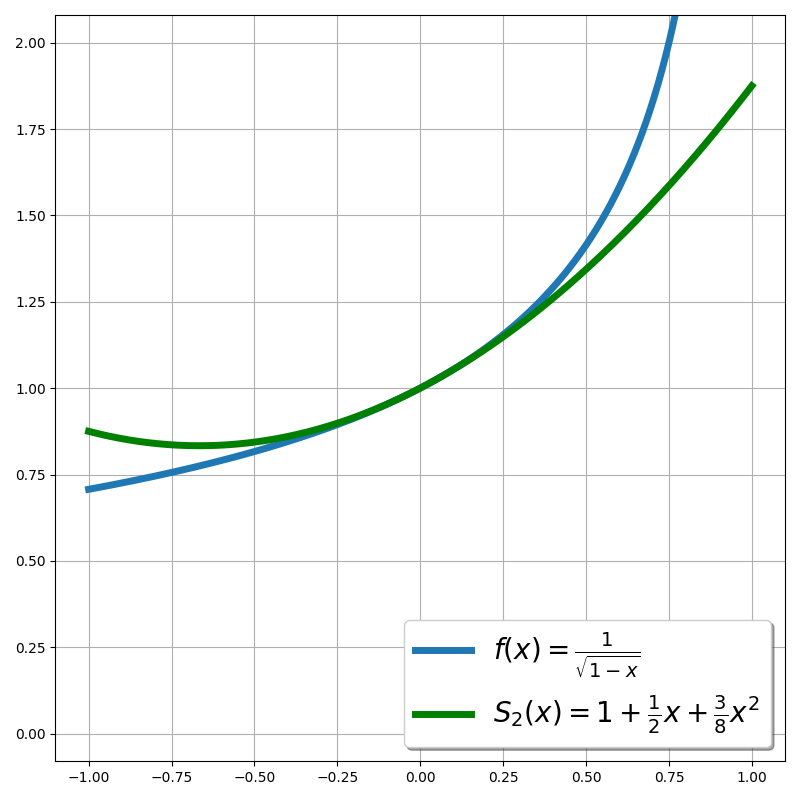
\includegraphics[width=0.8\textwidth]{UA_Section_8_3_Figure_1.png}
            \caption{\( f \) and \( S_2 \) on \( (-1, 1) \)}
            \label{fig:1}
        \end{figure}

        \item Using that
        \[
            f^{(N)}(t) = \frac{1 \cdot 3 \cdots (2n - 1)}{2^n} (1 - t)^{-n - 1/2}
        \]
        and Theorem 8.3.1, we have
        \begin{multline*}
            E_2(x) = \frac{1}{2} \int_0^x f^{(3)}(t) (x - t)^2 \, dt = \frac{1}{2} \int_0^x \frac{15}{8} (1 - t)^{-2 - 3/2} (x - t)^2 \, dt \\[2mm]
            = \frac{15}{16} \int_0^x \paren{\frac{x - t}{1 - t}}^2 \frac{1}{(1 - t)^{3/2}} \, dt.
        \end{multline*}
        
        \item First suppose that \( x \in [0, 1) \). The inequality \( 0 \leq t \leq x < 1 \) implies that
        \[
            t \geq xt \quimplies -t \leq -xt \quimplies x - t \leq x - xt = x (1 - t) \quimplies \frac{x - t}{1 - t} \leq x.
        \]
        Since \( \tfrac{x - t}{1 - t} \) and \( x \) are both non-negative in this case, we obtain the inequality \( \abs{\frac{x - t}{1 - t}} \leq \abs{x} \). Now suppose that \( x \in (-1, 0) \). The inequality \( -1 < x \leq t < 0 \) implies that
        \[
            1 \geq x \quimplies t \leq xt \quimplies t - x \leq xt - x = (-x)(1 - t) \quimplies \frac{t - x}{1 - t} \leq -x.
        \]
        Since \( \tfrac{x - t}{1 - t} \) and \( x \) are both negative in this case, we again obtain the inequality \( \abs{\frac{x - t}{1 - t}} \leq \abs{x} \).
        
        Using this inequality and the expression for \( E_2 \) found in part (b), we have for \( x \in [0, 1) \):
        \begin{align*}
            \abs{E_2(x)} &= \frac{15}{16} \abs{ \int_0^x \paren{\frac{x - t}{1 - t}}^2 \frac{1}{(1 - t)^{3/2}} \, dt } \\[2mm]
            &\leq \frac{15}{16} \int_0^x \abs{ \paren{\frac{x - t}{1 - t}}^2 \frac{1}{(1 - t)^{3/2}} } \, dt \\[2mm]
            &\leq \frac{15}{16} x^2 \int_0^x \frac{1}{(1 - t)^{3/2}} \, dt \\[2mm]
            &= \frac{15}{8} x^2 \bkt{\frac{1}{\sqrt{1 - t}}}^{t=x}_{t=0} \\[2mm]
            &= \frac{15}{8} x^2 \paren{ \frac{1}{\sqrt{1 - x}} - 1 }.
        \end{align*}
        Similarly, for \( x \in (-1, 0) \):
        \begin{align*}
            \abs{E_2(x)} &= \frac{15}{16} \abs{ \int_x^0 \paren{\frac{x - t}{1 - t}}^2 \frac{1}{(1 - t)^{3/2}} \, dt } \\[2mm]
            &\leq \frac{15}{16} x^2 \int_x^0 \frac{1}{(1 - t)^{3/2}} \, dt \\[2mm]
            &= \frac{15}{8} x^2 \bkt{\frac{1}{\sqrt{1 - t}}}^{t=0}_{t=x} \\[2mm]
            &= \frac{15}{8} x^2 \paren{ 1 - \frac{1}{\sqrt{1 - x}} }.
        \end{align*}
        Hence for all \( x \in (-1, 1) \) we have the overestimate
        \[
            \abs{E_2(x)} \leq \frac{15}{8} x^2 \abs{\frac{1}{\sqrt{1 - x}} - 1}.
        \]
        Denoting this overestimate by \( G(x) \) and comparing with the values from part (a), we find that
        \begin{gather*}
            E_2 \paren{\frac{1}{2}} \approx 0.0705 \leq 0.1942 \approx G \paren{\frac{1}{2}}, \\[2mm]
            E_2 \paren{\frac{3}{4}} \approx 0.4141 \leq 1.0547 \approx G \paren{\frac{3}{4}}, \\[2mm]
            E_2 \paren{\frac{8}{9}} \approx 1.2593 \leq 2.9630 \approx G \paren{\frac{8}{9}}.
        \end{gather*}

        \item Using that
        \[
            f^{(N)}(t) = \frac{1 \cdot 3 \cdots (2n - 1)}{2^n} (1 - t)^{-n - 1/2} = \frac{(2N)!}{2^{2N} N!} (1 - t)^{-N - 1/2}
        \]
        and Theorem 8.3.1, we have for a fixed \( x \in (-1, 1) \):
        \begin{multline*}
            E_N(x) = \frac{1}{N!} \int_0^x f^{(N+1)}(t) (x - t)^N \, dt = \frac{1}{N!} \cdot \frac{(2N + 2)!}{2^{2N + 2} (N + 1)!} \int_0^x \paren{\frac{x - t}{1 - t}}^N \frac{1}{(1 - t)^{3/2}} \, dt \\[2mm]
            = c_{N+1} (N + 1) \int_0^x \paren{\frac{x - t}{1 - t}}^N \frac{1}{(1 - t)^{3/2}} \, dt,
        \end{multline*}
        where \( (c_n) \) was defined in \Cref{ex:6}. From this expression we can derive, as in part (c), the estimate
        \[
            \abs{E_N(x)} \leq c_{N+1} (N + 1) \abs{x}^N \abs{\frac{1}{\sqrt{1 - x}} - 1}.
        \]
        Since \( \abs{x} < 1 \) we have \( \lim_{N \to \infty} (N + 1) \abs{x}^N = 0 \) and we showed in \Cref{ex:7} that \( \lim_{N \to \infty} c_{N+1} = 0 \); it now follows from the Squeeze Theorem that \( \lim_{n \to \infty} \abs{E_N(x)} = 0 \).
    \end{enumerate}
\end{solution}

\begin{exercise}
\label{ex:11}
    Assuming that the derivative of \( \arcsin(x) \) is indeed \( 1 / \sqrt{1 - x^2} \), supply the justification that allows us to conclude
    \makeatletter
    \tagsleft@true
    \begin{align*}
        \arcsin(x) = \sum_{n=0}^{\infty} \frac{c_n}{2n + 1} x^{2n + 1} \quad \text{for all } \abs{x} < 1 \, . \tag{5}
    \end{align*}
    \tagsleft@false
    \makeatother
\end{exercise}

\begin{solution}
    Because the power series \( \sum_{n=0}^{\infty} c_n x^{2n} \) converges to \( \tfrac{1}{\sqrt{1 - x^2}} \) on \( (-1, 1) \), \href{https://lew98.github.io/Mathematics/UA_Section_6_5_Exercises.pdf}{Exercise 6.5.4 (a)} shows that the power series
    \[
        \sum_{n=0}^{\infty} \frac{c_n}{2n + 1} x^{2n + 1}
    \]
    converges on \( (-1, 1) \) and has derivative \( \tfrac{1}{\sqrt{1 - x^2}} \). As this is also the derivative of \( \arcsin(x) \), Corollary 5.3.4 implies that
    \[
        \arcsin(x) = k + \sum_{n=0}^{\infty} \frac{c_n}{2n + 1} x^{2n + 1}
    \]
    for all \( x \in (-1, 1) \) and some \( k \in \R \); taking \( x = 0 \) shows that \( k = 0 \).
\end{solution}

\begin{exercise}
\label{ex:12}
    Our work thus far shows that the Taylor series in (5) is valid for all \( \abs{x} < 1 \), but note that \( \arcsin(x) \) is continuous for all \( \abs{x} \leq 1 \). Carefully explain why the series in (5) converges uniformly to \( \arcsin(x) \) on the closed interval \( [-1, 1] \).
\end{exercise}

\begin{solution}
    Letting \( a_n = \tfrac{2^{2n} (n!)^2}{(2n)! \sqrt{n}} \), we have
    \[
        \frac{c_n}{2n + 1} = \frac{a_n^{-1}}{\sqrt{n} (2n + 1)}
    \]
    for each \( n \in \N \). As \( (a_n) \) converges to \( \sqrt{\pi} \) (\Cref{ex:5}) and consists of strictly positive terms, there is some \( L > 0 \) such that \( a_n \geq L \) for all \( n \in \N \). It follows that
    \[
        \frac{c_n}{2n + 1} = \frac{a_n^{-1}}{\sqrt{n} (2n + 1)} \leq \frac{L^{-1}}{\sqrt{n} (2n + 1)}
    \]
    and hence the series \( \sum_{n=0}^{\infty} \tfrac{c_n}{2n + 1} \) converges by comparison with the series \( \sum_{n=1}^{\infty} \tfrac{1}{n^{3/2}} \). Since each term of the series \( \sum_{n=0}^{\infty} \tfrac{c_n}{2n + 1} \) is positive, we have shown that the power series \( \sum_{n=0}^{\infty} \frac{c_n}{2n + 1} x^{2n + 1} \) converges absolutely at \( x = 1 \); it follows from Theorem 6.5.2 that the convergence is uniform on \( [-1, 1] \). This implies that the power series is continuous on \( [-1, 1] \). Since \( \arcsin \) is also continuous on this interval, the function
    \[
        D(x) = \arcsin(x) - \sum_{n=0}^{\infty} \frac{c_n}{2n + 1} x^{2n + 1}
    \]
    is continuous on \( [-1, 1] \) and satisfies, by \Cref{ex:11}, \( D(x) = 0 \) for all \( x \in (-1, 1) \); by continuity, it must then be the case that \( D(-1) = D(1) = 0 \) also.
\end{solution}

\begin{exercise}
\label{ex:13}
    \begin{enumerate}
        \item Show
        \[
            \int_0^{\pi/2} \theta \, d\theta = \sum_{n=0}^{\infty} \frac{c_n}{2n + 1} b_{2n+1},
        \]
        being careful to justify each step in the argument. The term \( b_{2n+1} \) refers back to our earlier work on Wallis's product.

        \item Deduce
        \[
            \frac{\pi^2}{8} = \sum_{n=0}^{\infty} \frac{1}{(2n + 1)^2},
        \]
        and use this to finish the proof that \( \pi^2 / 6 = \sum_{n=1}^{\infty} 1 / n^2 \).
    \end{enumerate}
\end{exercise}

\begin{solution}
    \begin{enumerate}
        \item We have
        \[
            \int_0^{\pi/2} \theta \, d\theta = \int_0^{\pi/2} \paren{ \sum_{n=0}^{\infty} \frac{c_n}{2n + 1} \sin^{2n + 1}(\theta) } \, d\theta.
        \]
        The uniform convergence of \( \sum_{n=0}^{\infty} \frac{c_n}{2n + 1} \sin^{2n + 1}(\theta) \) on \( \bkt{-\tfrac{\pi}{2}, \tfrac{\pi}{2}} \), Theorem 7.4.4, and the linearity of the integral (Theorem 7.4.2 (i)) allow us to interchange the integral with the series, obtaining
        \[
            \int_0^{\pi/2} \theta \, d\theta = \sum_{n=0}^{\infty} \paren{ \int_0^{\pi/2} \frac{c_n}{2n + 1} \sin^{2n + 1}(\theta) \, d\theta } = \sum_{n=0}^{\infty} \frac{c_n}{2n + 1} b_{2n+1}.
        \]

        \item Using our formula for \( b_{2n+1} \) obtained in \Cref{ex:3} (c), we see that \( c_n b_{2n+1} = \tfrac{1}{2n + 1} \) and hence by part (a):
        \[
            \frac{\pi^2}{8} = \int_0^{\pi/2} \theta \, d\theta = \sum_{n=0}^{\infty} \frac{c_n}{2n + 1} b_{2n+1} = \sum_{n=0}^{\infty} \frac{1}{(2n + 1)^2}.
        \]
        Now we split the sum \( \sum_{n=1}^{\infty} \tfrac{1}{n^2} \) over the odd and even positive integers:
        \[
            \sum_{n=1}^{\infty} \frac{1}{n^2} = \sum_{n=0}^{\infty} \frac{1}{(2n + 1)^2} + \sum_{n=1}^{\infty} \frac{1}{(2n)^2} = \frac{\pi^2}{8} + \frac{1}{4} \sum_{n=1}^{\infty} \frac{1}{n^2};
        \]
        these manipulations are valid because these are convergent series. It follows from the above expression that
        \[
            \sum_{n=1}^{\infty} \frac{1}{n^2} = \frac{\pi^2}{6}.
        \]
    \end{enumerate}
\end{solution}

\noindent \hrulefill

\noindent \hypertarget{ua}{\textcolor{blue}{[UA]} Abbott, S. (2015) \textit{Understanding Analysis.} 2\ts{nd} edition.}

\end{document}